

\documentclass[journal, twoside]{IEEEtran}
% *** CITATION PACKAGES ***
%

%\usepackage[brazilian]{babel}%%%%% for papers in portuguese
%\usepackage[spanish]{babel}%%%%% for papers in Spanish
\usepackage{fancyhdr} %used for header
\pagestyle{fancy} %also used for header
\usepackage{lipsum}
\usepackage[utf8]{inputenc}
\usepackage[T1]{fontenc}

\usepackage{graphicx}
\usepackage{subcaption}

\usepackage{graphicx} %% for loading jpg figures
\usepackage{subfig}
\usepackage{nccmath}
\usepackage{color}
\usepackage{cite}
\usepackage{acro}
\usepackage{scalerel}
\usepackage{tikz}
\usetikzlibrary{svg.path}

\definecolor{orcidlogocol}{HTML}{A6CE39}
\tikzset{
  orcidlogo/.pic={
    \fill[orcidlogocol] svg{M256,128c0,70.7-57.3,128-128,128C57.3,256,0,198.7,0,128C0,57.3,57.3,0,128,0C198.7,0,256,57.3,256,128z};
    \fill[white] svg{M86.3,186.2H70.9V79.1h15.4v48.4V186.2z}
                 svg{M108.9,79.1h41.6c39.6,0,57,28.3,57,53.6c0,27.5-21.5,53.6-56.8,53.6h-41.8V79.1z M124.3,172.4h24.5c34.9,0,42.9-26.5,42.9-39.7c0-21.5-13.7-39.7-43.7-39.7h-23.7V172.4z}
                 svg{M88.7,56.8c0,5.5-4.5,10.1-10.1,10.1c-5.6,0-10.1-4.6-10.1-10.1c0-5.6,4.5-10.1,10.1-10.1C84.2,46.7,88.7,51.3,88.7,56.8z};
  }
}

\newcommand\orcidicon[1]{\href{https://orcid.org/#1}{\mbox{\scalerel*{

\begin{tikzpicture}[yscale=-1,transform shape]
\pic{orcidlogo};
\end{tikzpicture}
}{|}}}}



%%%% Page headears


%%% header 1st page, still does not work

%\fancypagestyle{firstpage}{%
 % \lhead{IEEE LATIN AMERICA TRANSACTIONS ,~Vol.~7, No.~7, Oct~2020*}
 % \rhead{\thepage}
%}


\renewcommand{\headrulewidth}{0pt}% disable the underline of the header part

% cite.sty was written by Donald Arseneau
% V1.6 and later of IEEEtran pre-defines the format of the cite.sty package
% \cite{} output to follow that of the IEEE. Loading the cite package will
% result in citation numbers being automatically sorted and properly
% "compressed/ranged". e.g., [1], [9], [2], [7], [5], [6] without using
% cite.sty will become [1], [2], [5]--[7], [9] using cite.sty. cite.sty's
% \cite will automatically add leading space, if needed. Use cite.sty's
% noadjust option (cite.sty V3.8 and later) if you want to turn this off
% such as if a citation ever needs to be enclosed in parenthesis.
% cite.sty is already installed on most LaTeX systems. Be sure and use
% version 5.0 (2009-03-20) and later if using hyperref.sty.
% The latest version can be obtained at:
% http://www.ctan.org/pkg/cite
% The documentation is contained in the cite.sty file itself.






% *** GRAPHICS RELATED PACKAGES ***
%
\ifCLASSINFOpdf
  % \usepackage[pdftex]{graphicx}
  % declare the path(s) where your graphic files are
  % \graphicspath{{../pdf/}{../jpeg/}}
  % and their extensions so you won't have to specify these with
  % every instance of \includegraphics
  % \DeclareGraphicsExtensions{.pdf,.jpeg,.png}
\else
  % or other class option (dvipsone, dvipdf, if not using dvips). graphicx
  % will default to the driver specified in the system graphics.cfg if no
  % driver is specified.
  % \usepackage[dvips]{graphicx}
  % declare the path(s) where your graphic files are
  % \graphicspath{{../eps/}}
  % and their extensions so you won't have to specify these with
  % every instance of \includegraphics
  % \DeclareGraphicsExtensions{.eps}
\fi
% graphicx was written by David Carlisle and Sebastian Rahtz. It is
% required if you want graphics, photos, etc. graphicx.sty is already
% installed on most LaTeX systems. The latest version and documentation
% can be obtained at: 
% http://www.ctan.org/pkg/graphicx
% Another good source of documentation is "Using Imported Graphics in
% LaTeX2e" by Keith Reckdahl which can be found at:
% http://www.ctan.org/pkg/epslatex
%
% latex, and pdflatex in dvi mode, support graphics in encapsulated
% postscript (.eps) format. pdflatex in pdf mode supports graphics
% in .pdf, .jpeg, .png and .mps (metapost) formats. Users should ensure
% that all non-photo figures use a vector format (.eps, .pdf, .mps) and
% not a bitmapped formats (.jpeg, .png). The IEEE frowns on bitmapped formats
% which can result in "jaggedy"/blurry rendering of lines and letters as
% well as large increases in file sizes.
%
% You can find documentation about the pdfTeX application at:
% http://www.tug.org/applications/pdftex





% *** MATH PACKAGES ***
%
%\usepackage{amsmath}
% A popular package from the American Mathematical Society that provides
% many useful and powerful commands for dealing with mathematics.
%
% Note that the amsmath package sets \interdisplaylinepenalty to 10000
% thus preventing page breaks from occurring within multiline equations. Use:
%\interdisplaylinepenalty=2500
% after loading amsmath to restore such page breaks as IEEEtran.cls normally
% does. amsmath.sty is already installed on most LaTeX systems. The latest
% version and documentation can be obtained at:
% http://www.ctan.org/pkg/amsmath





% *** SPECIALIZED LIST PACKAGES ***
%
%\usepackage{algorithmic}
% algorithmic.sty was written by Peter Williams and Rogerio Brito.
% This package provides an algorithmic environment fo describing algorithms.
% You can use the algorithmic environment in-text or within a figure
% environment to provide for a floating algorithm. Do NOT use the algorithm
% floating environment provided by algorithm.sty (by the same authors) or
% algorithm2e.sty (by Christophe Fiorio) as the IEEE does not use dedicated
% algorithm float types and packages that provide these will not provide
% correct IEEE style captions. The latest version and documentation of
% algorithmic.sty can be obtained at:
% http://www.ctan.org/pkg/algorithms
% Also of interest may be the (relatively newer and more customizable)
% algorithmicx.sty package by Szasz Janos:
% http://www.ctan.org/pkg/algorithmicx




% *** ALIGNMENT PACKAGES ***
%
%\usepackage{array}
% Frank Mittelbach's and David Carlisle's array.sty patches and improves
% the standard LaTeX2e array and tabular environments to provide better
% appearance and additional user controls. As the default LaTeX2e table
% generation code is lacking to the point of almost being broken with
% respect to the quality of the end results, all users are strongly
% advised to use an enhanced (at the very least that provided by array.sty)
% set of table tools. array.sty is already installed on most systems. The
% latest version and documentation can be obtained at:
% http://www.ctan.org/pkg/array


% IEEEtran contains the IEEEeqnarray family of commands that can be used to
% generate multiline equations as well as matrices, tables, etc., of high
% quality.




% *** SUBFIGURE PACKAGES ***
%\ifCLASSOPTIONcompsoc
%  \usepackage[caption=false,font=normalsize,labelfont=sf,textfont=sf]{subfig}
%\else
%  \usepackage[caption=false,font=footnotesize]{subfig}
%\fi
% subfig.sty, written by Steven Douglas Cochran, is the modern replacement
% for subfigure.sty, the latter of which is no longer maintained and is
% incompatible with some LaTeX packages including fixltx2e. However,
% subfig.sty requires and automatically loads Axel Sommerfeldt's caption.sty
% which will override IEEEtran.cls' handling of captions and this will result
% in non-IEEE style figure/table captions. To prevent this problem, be sure
% and invoke subfig.sty's "caption=false" package option (available since
% subfig.sty version 1.3, 2005/06/28) as this is will preserve IEEEtran.cls
% handling of captions.
% Note that the Computer Society format requires a larger sans serif font
% than the serif footnote size font used in traditional IEEE formatting
% and thus the need to invoke different subfig.sty package options depending
% on whether compsoc mode has been enabled.
%
% The latest version and documentation of subfig.sty can be obtained at:
% http://www.ctan.org/pkg/subfig




% *** FLOAT PACKAGES ***
%
%\usepackage{fixltx2e}
% fixltx2e, the successor to the earlier fix2col.sty, was written by
% Frank Mittelbach and David Carlisle. This package corrects a few problems
% in the LaTeX2e kernel, the most notable of which is that in current
% LaTeX2e releases, the ordering of single and double column floats is not
% guaranteed to be preserved. Thus, an unpatched LaTeX2e can allow a
% single column figure to be placed prior to an earlier double column
% figure.
% Be aware that LaTeX2e kernels dated 2015 and later have fixltx2e.sty's
% corrections already built into the system in which case a warning will
% be issued if an attempt is made to load fixltx2e.sty as it is no longer
% needed.
% The latest version and documentation can be found at:
% http://www.ctan.org/pkg/fixltx2e


%\usepackage{stfloats}
% stfloats.sty was written by Sigitas Tolusis. This package gives LaTeX2e
% the ability to do double column floats at the bottom of the page as well
% as the top. (e.g., "\begin{figure*}[!b]" is not normally possible in
% LaTeX2e). It also provides a command:
%\fnbelowfloat
% to enable the placement of footnotes below bottom floats (the standard
% LaTeX2e kernel puts them above bottom floats). This is an invasive package
% which rewrites many portions of the LaTeX2e float routines. It may not work
% with other packages that modify the LaTeX2e float routines. The latest
% version and documentation can be obtained at:
% http://www.ctan.org/pkg/stfloats
% Do not use the stfloats baselinefloat ability as the IEEE does not allow
% \baselineskip to stretch. Authors submitting work to the IEEE should note
% that the IEEE rarely uses double column equations and that authors should try
% to avoid such use. Do not be tempted to use the cuted.sty or midfloat.sty
% packages (also by Sigitas Tolusis) as the IEEE does not format its papers in
% such ways.
% Do not attempt to use stfloats with fixltx2e as they are incompatible.
% Instead, use Morten Hogholm'a dblfloatfix which combines the features
% of both fixltx2e and stfloats:
%
% \usepackage{dblfloatfix}
% The latest version can be found at:
% http://www.ctan.org/pkg/dblfloatfix




%\ifCLASSOPTIONcaptionsoff
%  \usepackage[nomarkers]{endfloat}
% \let\MYoriglatexcaption\caption
% \renewcommand{\caption}[2][\relax]{\MYoriglatexcaption[#2]{#2}}
%\fi
% endfloat.sty was written by James Darrell McCauley, Jeff Goldberg and 
% Axel Sommerfeldt. This package may be useful when used in conjunction with 
% IEEEtran.cls'  captionsoff option. Some IEEE journals/societies require that
% submissions have lists of figures/tables at the end of the paper and that
% figures/tables without any captions are placed on a page by themselves at
% the end of the document. If needed, the draftcls IEEEtran class option or
% \CLASSINPUTbaselinestretch interface can be used to increase the line
% spacing as well. Be sure and use the nomarkers option of endfloat to
% prevent endfloat from "marking" where the figures would have been placed
% in the text. The two hack lines of code above are a slight modification of
% that suggested by in the endfloat docs (section 8.4.1) to ensure that
% the full captions always appear in the list of figures/tables - even if
% the user used the short optional argument of \caption[]{}.
% IEEE papers do not typically make use of \caption[]'s optional argument,
% so this should not be an issue. A similar trick can be used to disable
% captions of packages such as subfig.sty that lack options to turn off
% the subcaptions:
% For subfig.sty:
% \let\MYorigsubfloat\subfloat
% \renewcommand{\subfloat}[2][\relax]{\MYorigsubfloat[]{#2}}
% However, the above trick will not work if both optional arguments of
% the \subfloat command are used. Furthermore, there needs to be a
% description of each subfigure *somewhere* and endfloat does not add
% subfigure captions to its list of figures. Thus, the best approach is to
% avoid the use of subfigure captions (many IEEE journals avoid them anyway)
% and instead reference/explain all the subfigures within the main caption.
% The latest version of endfloat.sty and its documentation can obtained at:
% http://www.ctan.org/pkg/endfloat
%
% The IEEEtran \ifCLASSOPTIONcaptionsoff conditional can also be used
% later in the document, say, to conditionally put the References on a 
% page by themselves.




% *** PDF, URL AND HYPERLINK PACKAGES ***
%
%\usepackage{url}
% url.sty was written by Donald Arseneau. It provides better support for
% handling and breaking URLs. url.sty is already installed on most LaTeX
% systems. The latest version and documentation can be obtained at:
% http://www.ctan.org/pkg/url
% Basically, \url{my_url_here}.




% *** Do not adjust lengths that control margins, column widths, etc. ***
% *** Do not use packages that alter fonts (such as pslatex).         ***
% There should be no need to do such things with IEEEtran.cls V1.6 and later.
% (Unless specifically asked to do so by the journal or conference you plan
% to submit to, of course. )


% correct bad hyphenation here
\hyphenation{op-tical net-works semi-conduc-tor}

\DeclareAcronym{acm}{
  short = ACM ,
  long  = Association for Computing Machinery ,
  sort  = A ,
}


\usepackage{hyperref} %<--- Load after everything else
\begin{document}
 

 \setcounter{page}{0}%%%% HERE SET THE PAGE NUMBER
% \thispagestyle{firstpage}
%
% paper title
% Titles are generally capitalized except for words such as a, an, and, as,
% at, but, by, for, in, nor, of, on, or, the, to and up, which are usually
% not capitalized unless they are the first or last word of the title.
% Linebreaks \\ can be used within to get better formatting as desired.
% Do not put math or special symbols in the title.
\title{Avaliação de Desempenho em Sequencial e Paralelo}
%
%
% author names and IEEE memberships
% note positions of commas and nonbreaking spaces ( ~ ) LaTeX will not break
% a structure at a ~ so this keeps an author's name from being broken across
% two lines.
% use \thanks{} to gain access to the first footnote area
% a separate \thanks must be used for each paragraph as LaTeX2e's \thanks
% was not built to handle multiple paragraphs
%

\author{Kananda C V da Silva RA116382, Vitor H S de Camargo Ra116426, Natalia M Oyama Ra112652
% <-this % stops a space
\thanks{}% <-this % stops a space
\thanks{}% <-this % stops a space
\thanks{}
}





% The paper headers
%\markboth{IEEE Latin America Transactions,~Vol.~14, No.~8, August~2021}{Shell \MakeLowercase{\textit{et al.}}: Bare Demo of IEEEtran.cls for IEEE Journals}

%\markboth{left head}{}
%\markright{right head}
%\rhead{right head}
%\lhead{Left head}

\  
% The only time the second header will appear is for the odd numbered pages
% after the title page when using the twoside option.
% 
% *** Note that you probably will NOT want to include the author's ***
% *** name in the headers of peer review papers.                   ***
% You can use \ifCLASSOPTIONpeerreview for conditional compilation here if
% you desire.




% If you want to put a publisher's ID mark on the page you can do it like
% this:
%\IEEEpubid{0000--0000/00\$00.00~\copyright~2015 IEEE}
% Remember, if you use this you must call \IEEEpubidadjcol in the second
% column for its text to clear the IEEEpubid mark.



% use for special paper notices
%\IEEEspecialpapernotice{(Invited Paper)}




% make the title area
\maketitle

\IEEEpeerreviewmaketitle



\section{Introdução}

\par \quad Este trabalho tem como objetivo a implementação e coleta de dados de execução para análise de matrizes, tanto de forma sequencial como paralela.
\par \quad O primeiro código, “singlethread.c”, implementa uma forma de multiplicação de matrizes simples, sem utilizar paralelismo. O paralelismo utilizado neste código serve somente para o preenchimento da matriz alocada dinamicamente, uma vez que os objetivos são obter o speedup da multiplicação de matrizes somente, não havendo necessidade de incluir o tempo do preenchimento. 
\par \quad O segundo código, “multithread.c”, implementa tanto o paralelismo no preenchimento das matrizes como na multiplicação das mesmas. O paralelismo escolhido foi o paralelismo de dados, pois assim cada thread poderá executar o mesmo código de multiplicação em partes diferentes do código.



% \cite{koroishi2015robust,koroishi2016robust,yang2018networked},  \cite{liu2018dynamic,liang2017optimal},  \cite{luo2018active,koroishi2014numerical}  \cite{nugraha2018setting} 


\section{multiplicação em paralelo}
\par \quad Para a implementação do paralelismo, foi utilizado como base o código anteriormente feito “singlethread.c”, aplicando técnicas de paralelismo onde se fez necessário. A principal diferença entre os dois códigos se dá no comando for da linguagem C que percorre a matriz. 
\par \quad Enquanto na versão singlethread um único thread percorre todas as linhas e colunas da matriz efetuando a multiplicação, na versão paralelizada, cada thread executa linhas específicas da matriz de acordo com seu identificador passado na criação do thread com o comando pthread create. Ou seja, supondo que temos 10 threads criadas, a thread identificada como thread 0 irá executar as linhas 0, 10, 20, 30 e assim por diante, enquanto a thread 1 irá executar as linhas 1, 11, 21, 31 etc. da matriz. Portanto, cada thread começa os cálculos na linha de seu identificador e a variável de controle é incrementada de acordo com o número total de threads criadas.



\section{Results}


\par \quad As configurações das máquinas utilizadas para obtenção dos dados se encontram na tabela 1.
\newline \newline
%\begin{figure}[!t]
\centering
\subfloat{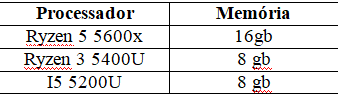
\includegraphics[width=2.5in]{tabela.png}}%
\newline Tabela 1. Configurações utilizadas.
\label{fig:bancada}
\hfil
\subfloat{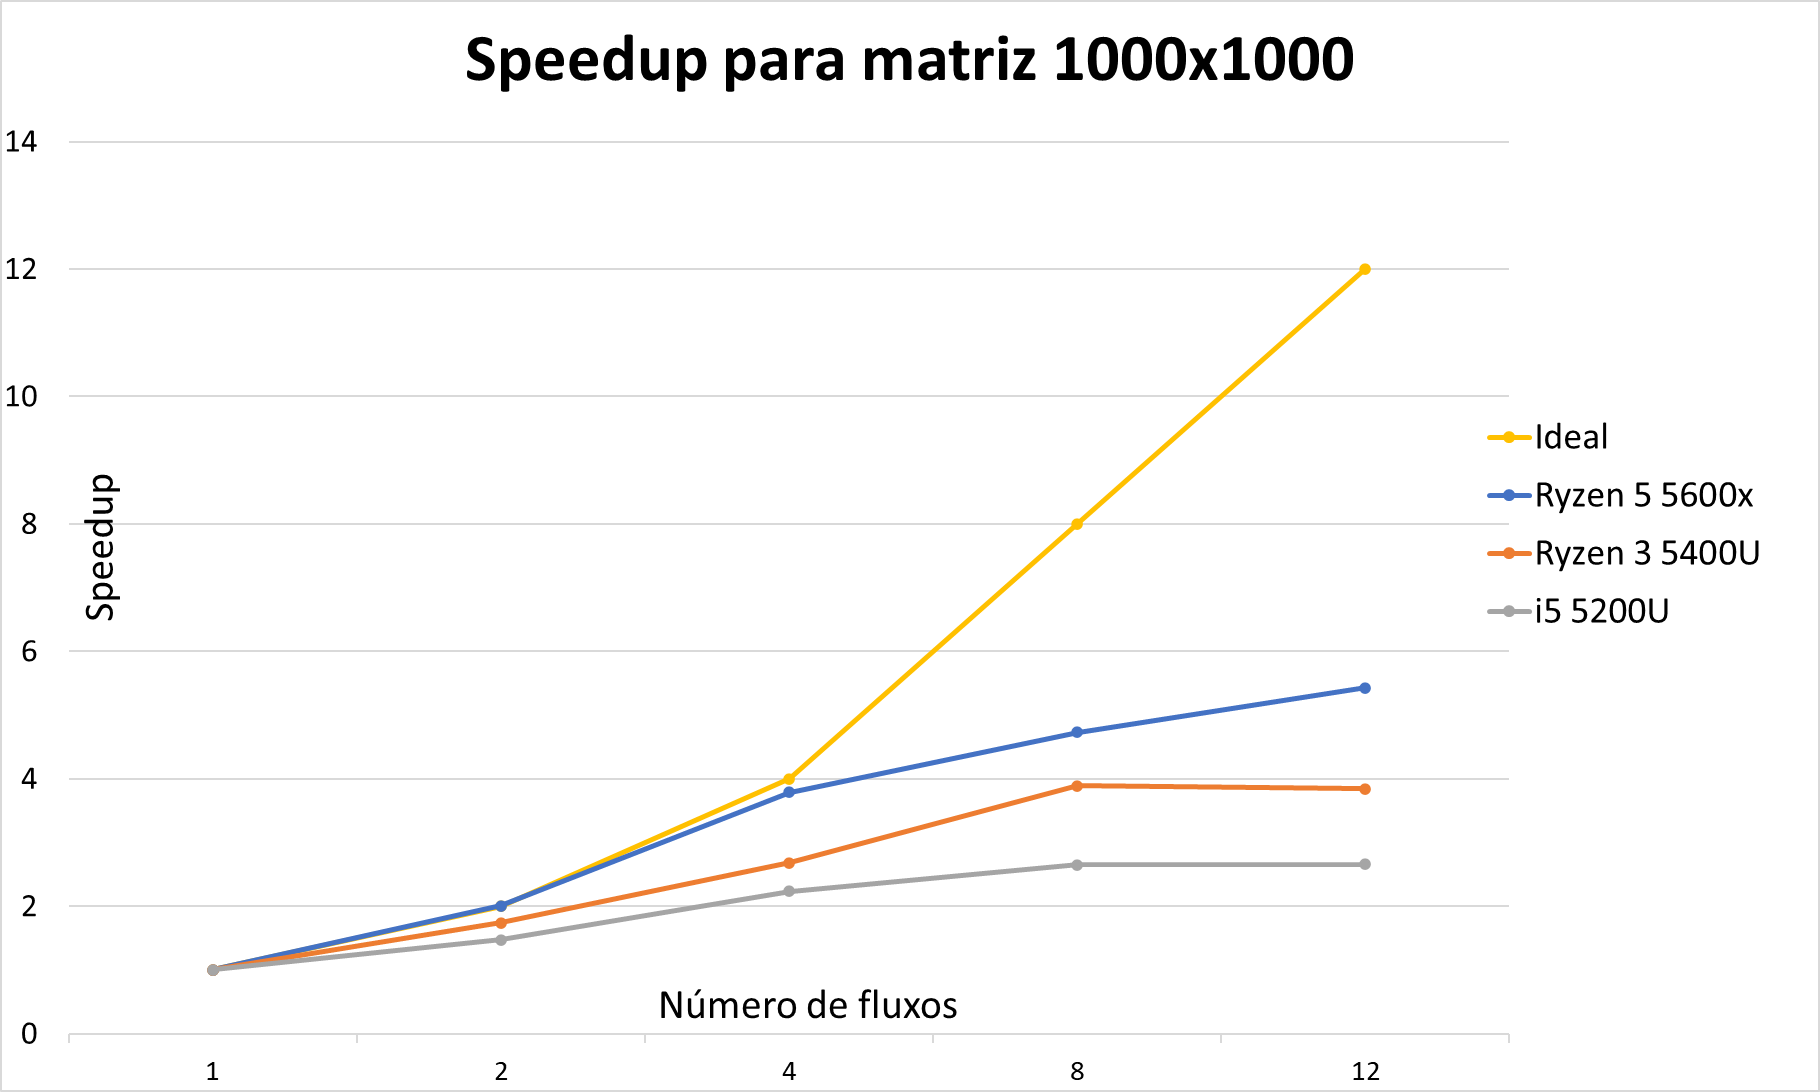
\includegraphics[width=2.5in]{speedup-1000.png}}%
\newline Figura 1. Gráfico speedup para matriz de tamanho 1000.
\label{fig:diagrama}

\label{fig:est}
\hfil
\subfloat{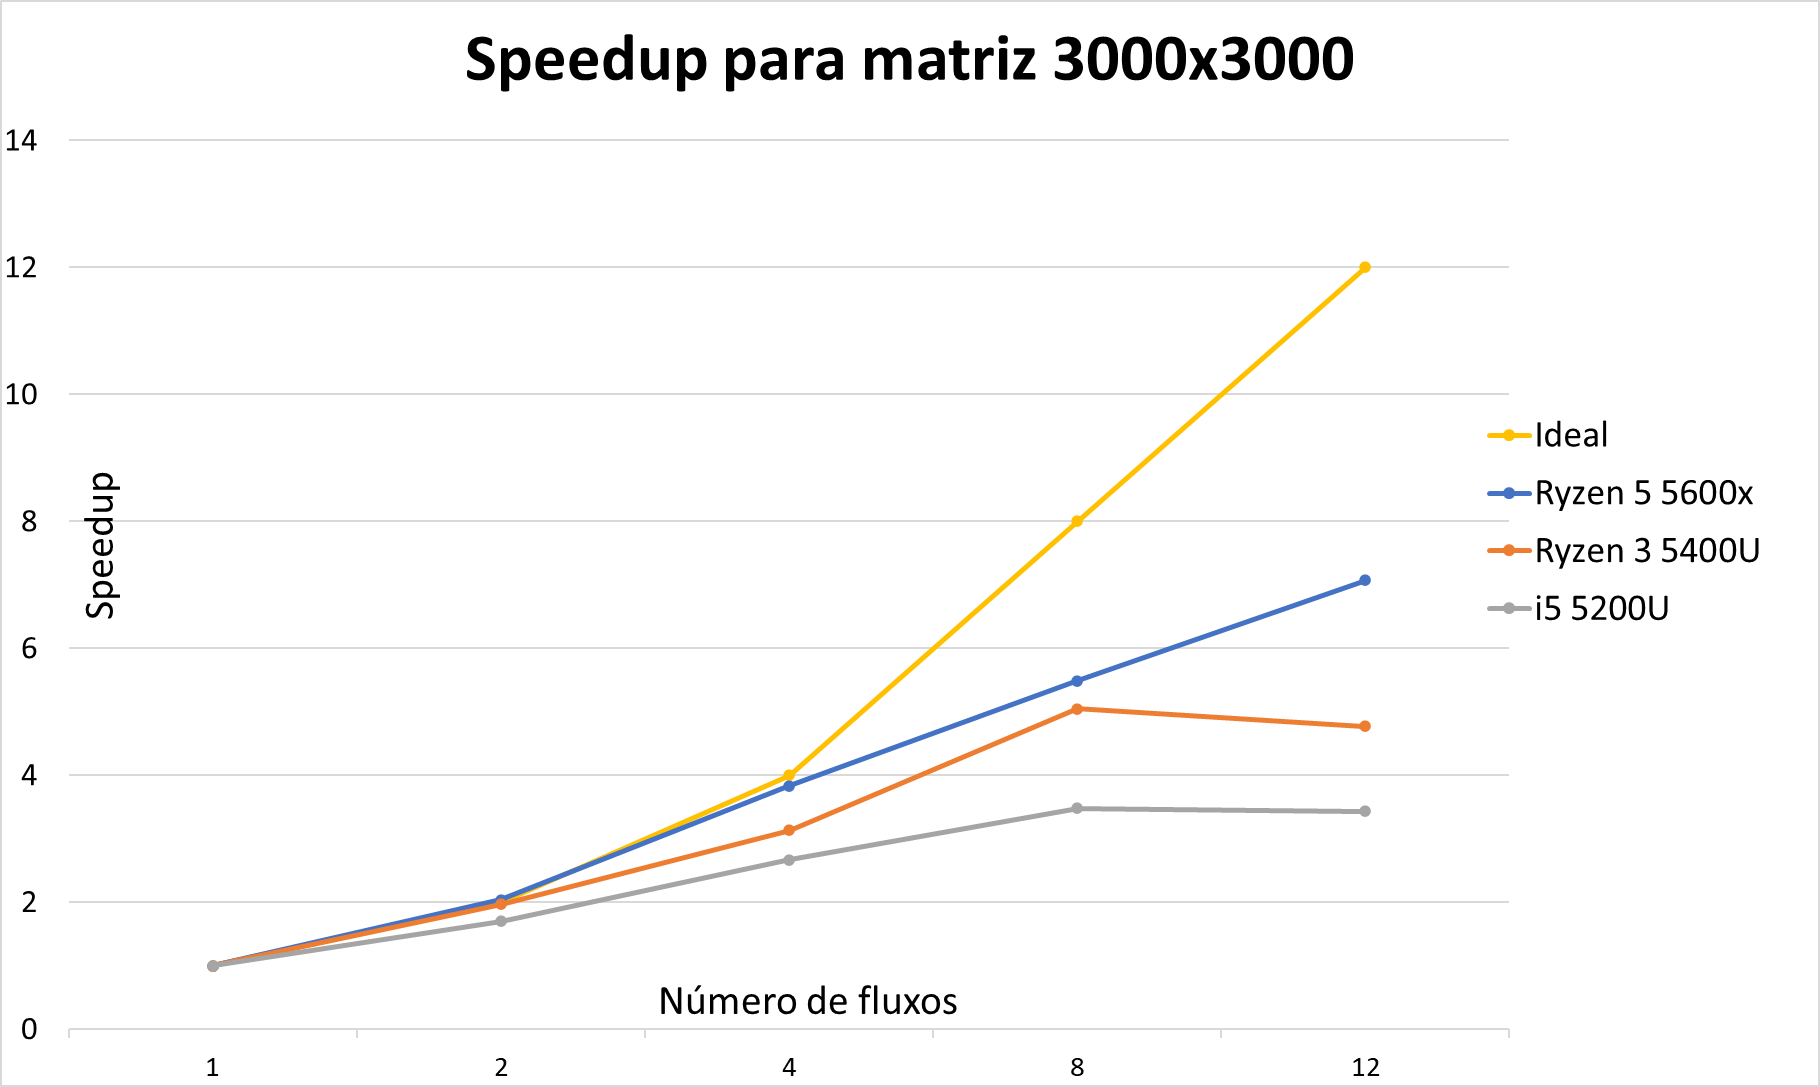
\includegraphics[width=2.5in]{speedup-3000.png}}%
\newline Figura 2. Gráfico speedup para matriz de tamanho 5000.
\label{fig:diagrama}

\label{fig:est}
\hfil
\subfloat{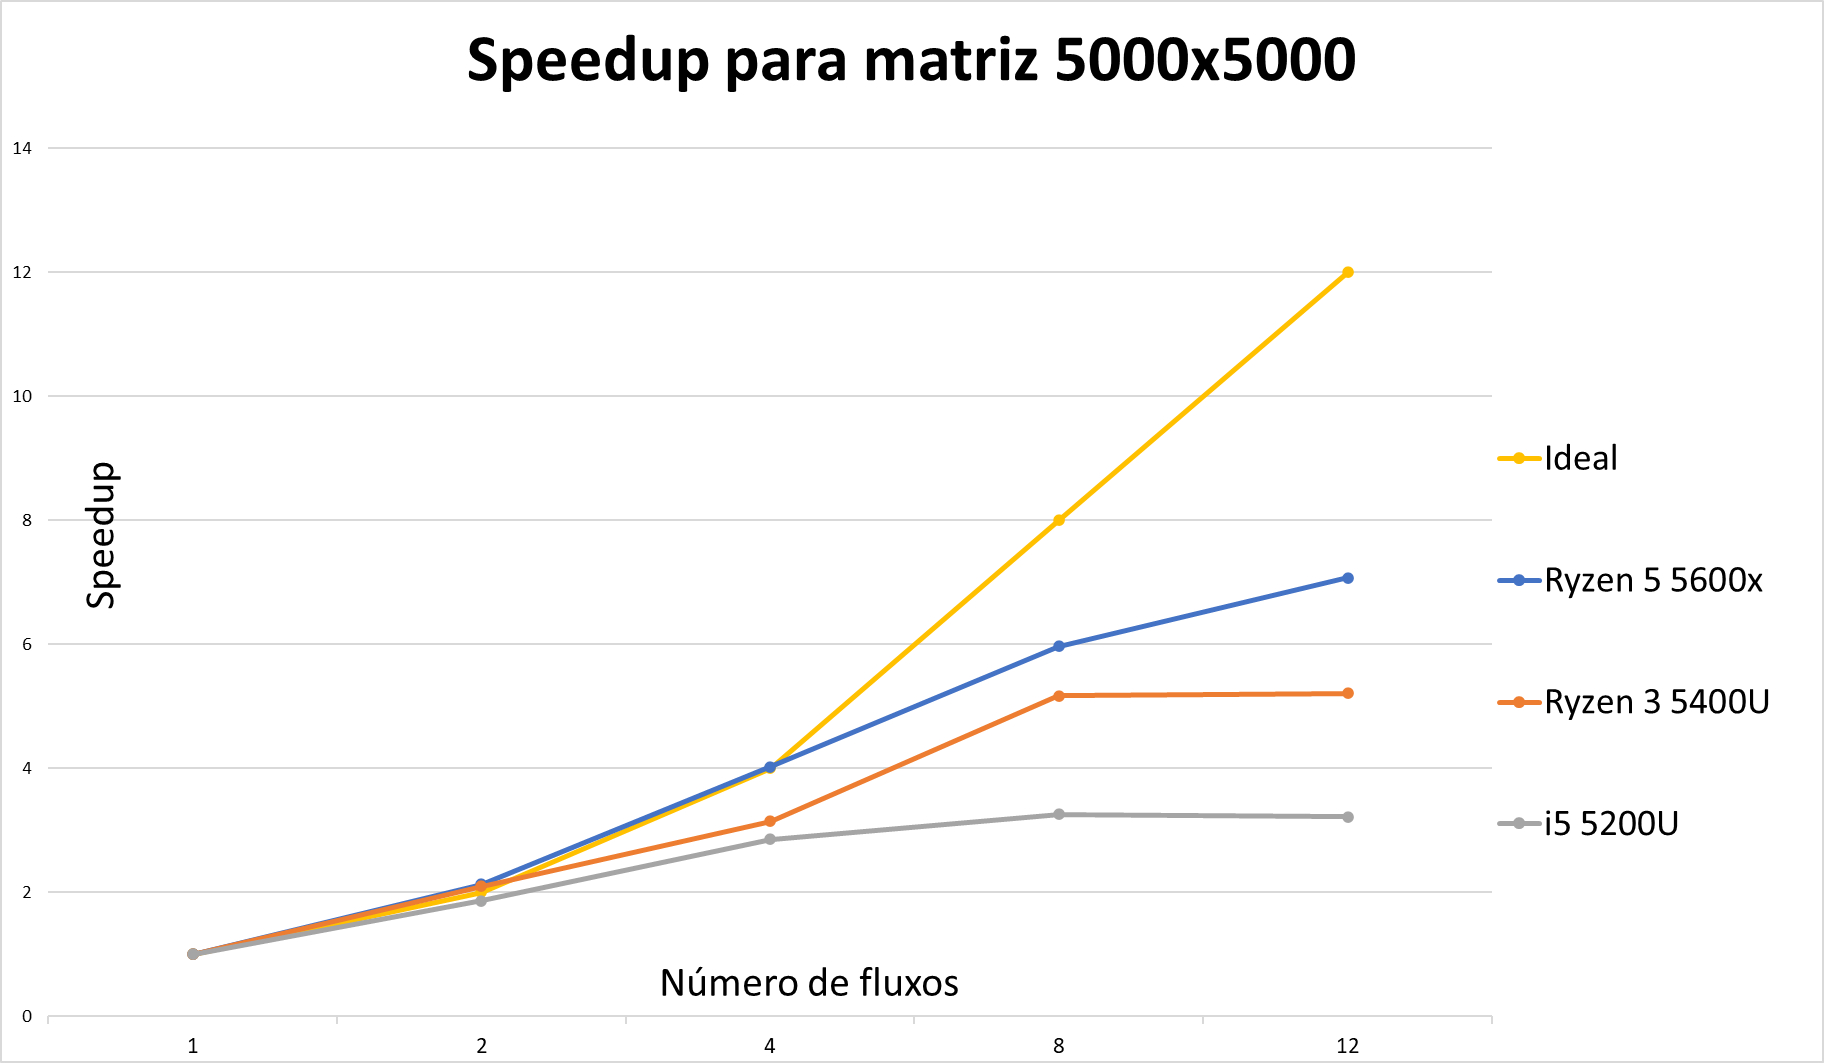
\includegraphics[width=2.5in]{speedup-5000.png}}%
\newline Figura 2. Gráfico speedup para matriz de tamanho 5000.
\label{fig:diagrama}

\label{fig:est}
\hfil
\label{fig:est}
\hfil
\subfloat{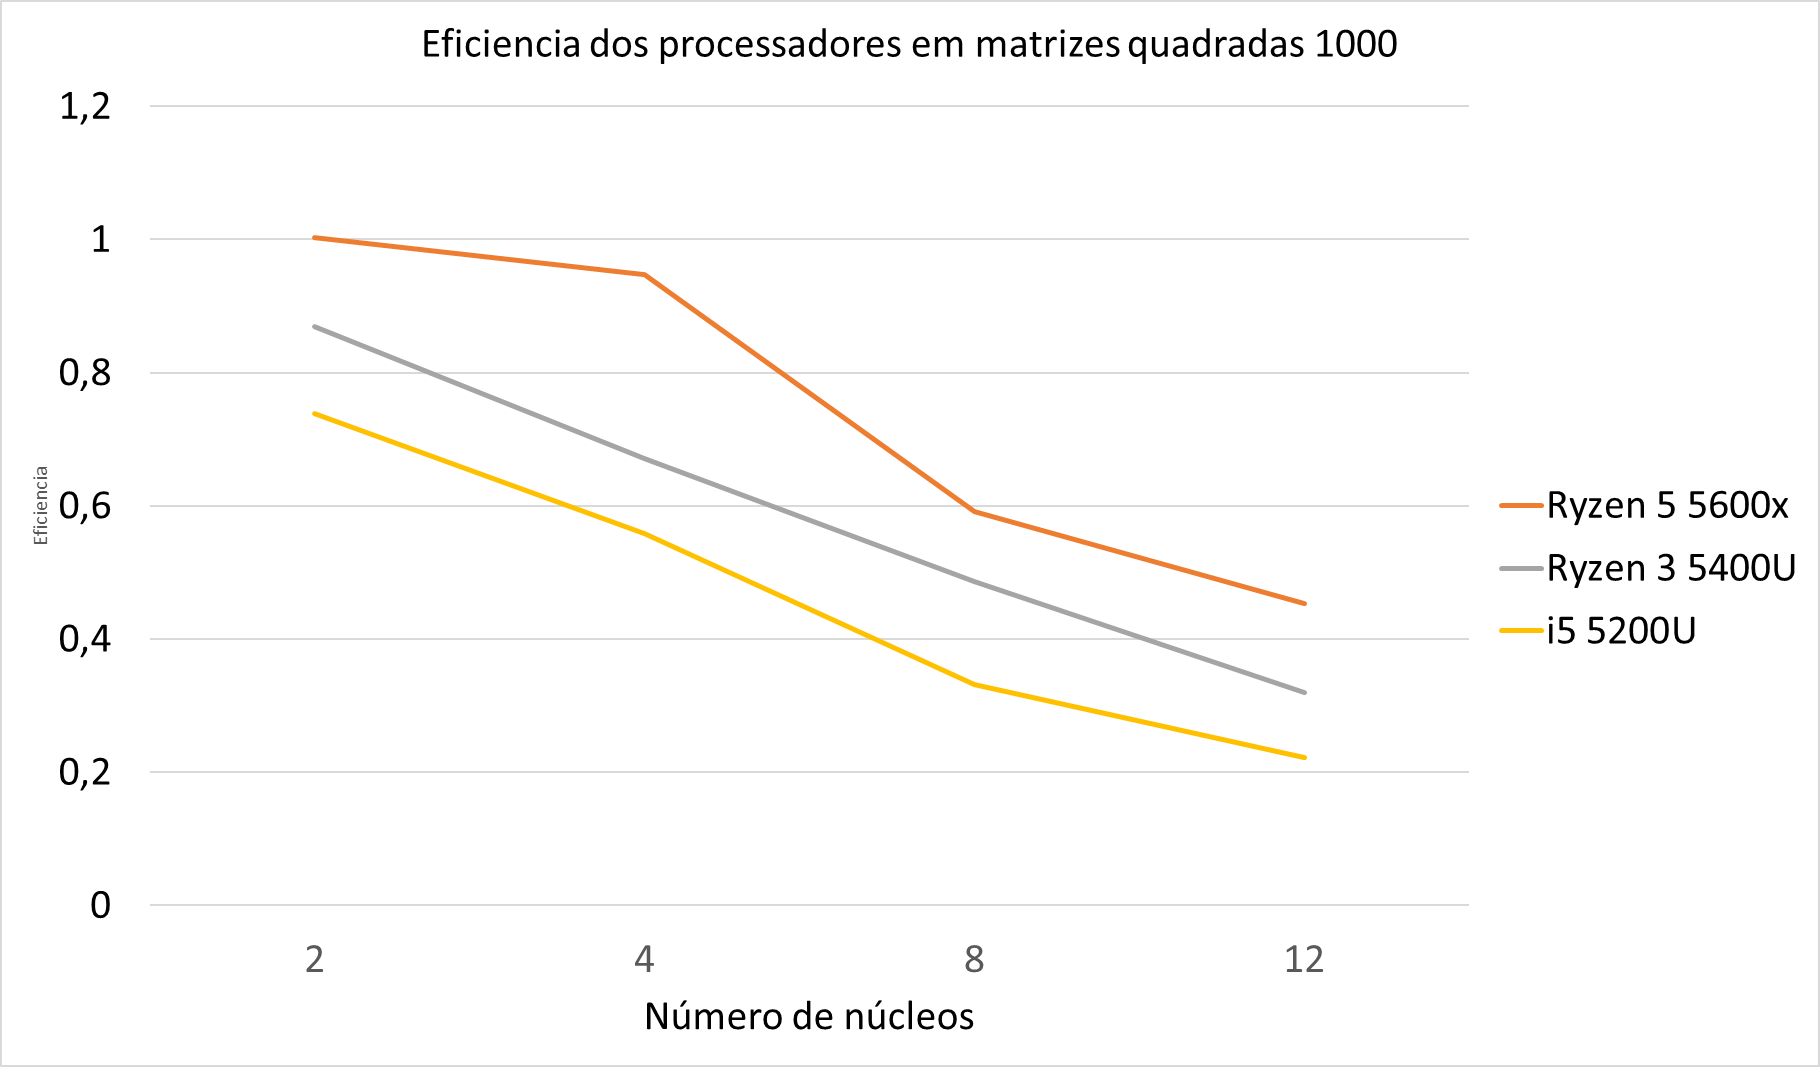
\includegraphics[width=2.5in]{eficiencia-1000.png}}%
\newline Figura 3. Gráfico de eficiência de cada processador para matriz de tamanho 1000.
\label{fig:diagrama}

\label{fig:est}
\hfil
\label{fig:est}
\hfil
\subfloat{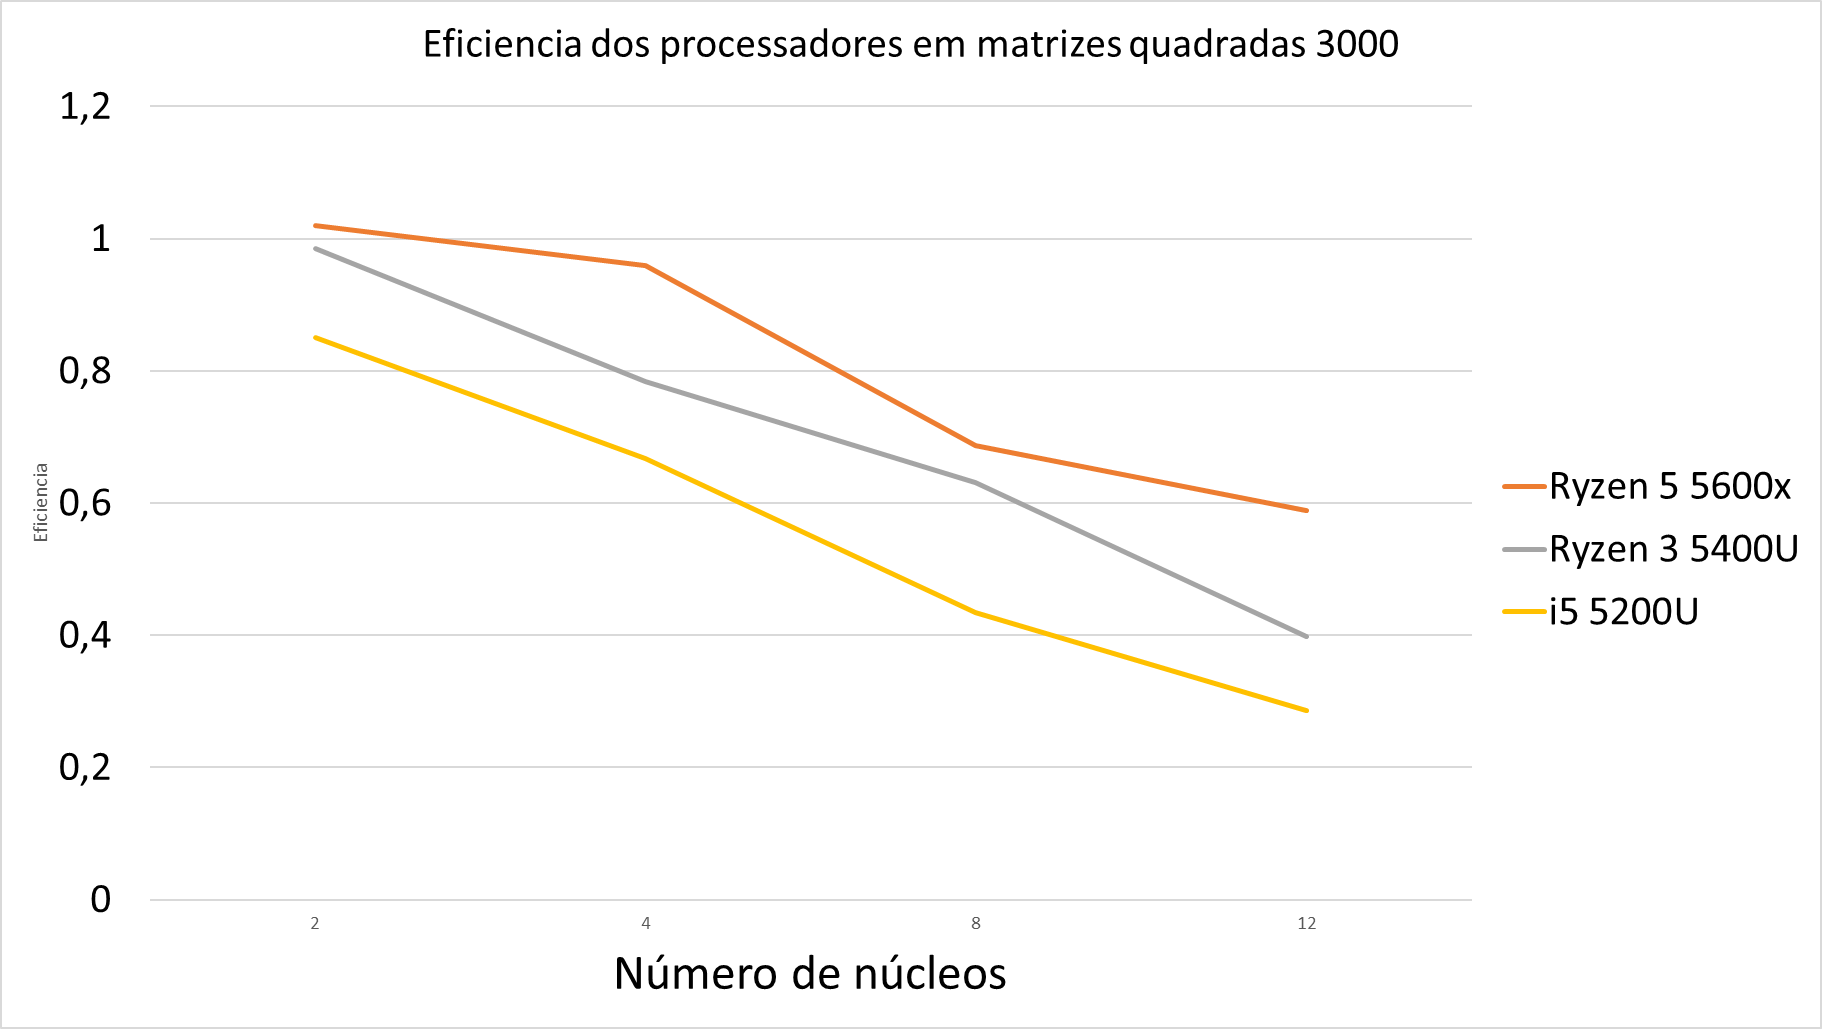
\includegraphics[width=2.5in]{eficiencia-3000.png}}%
\newline Figura 4. Gráfico de eficiência de cada processador para matriz de tamanho 3000
\label{fig:diagrama}

\label{fig:est}
\hfil
\label{fig:est}

\subfloat{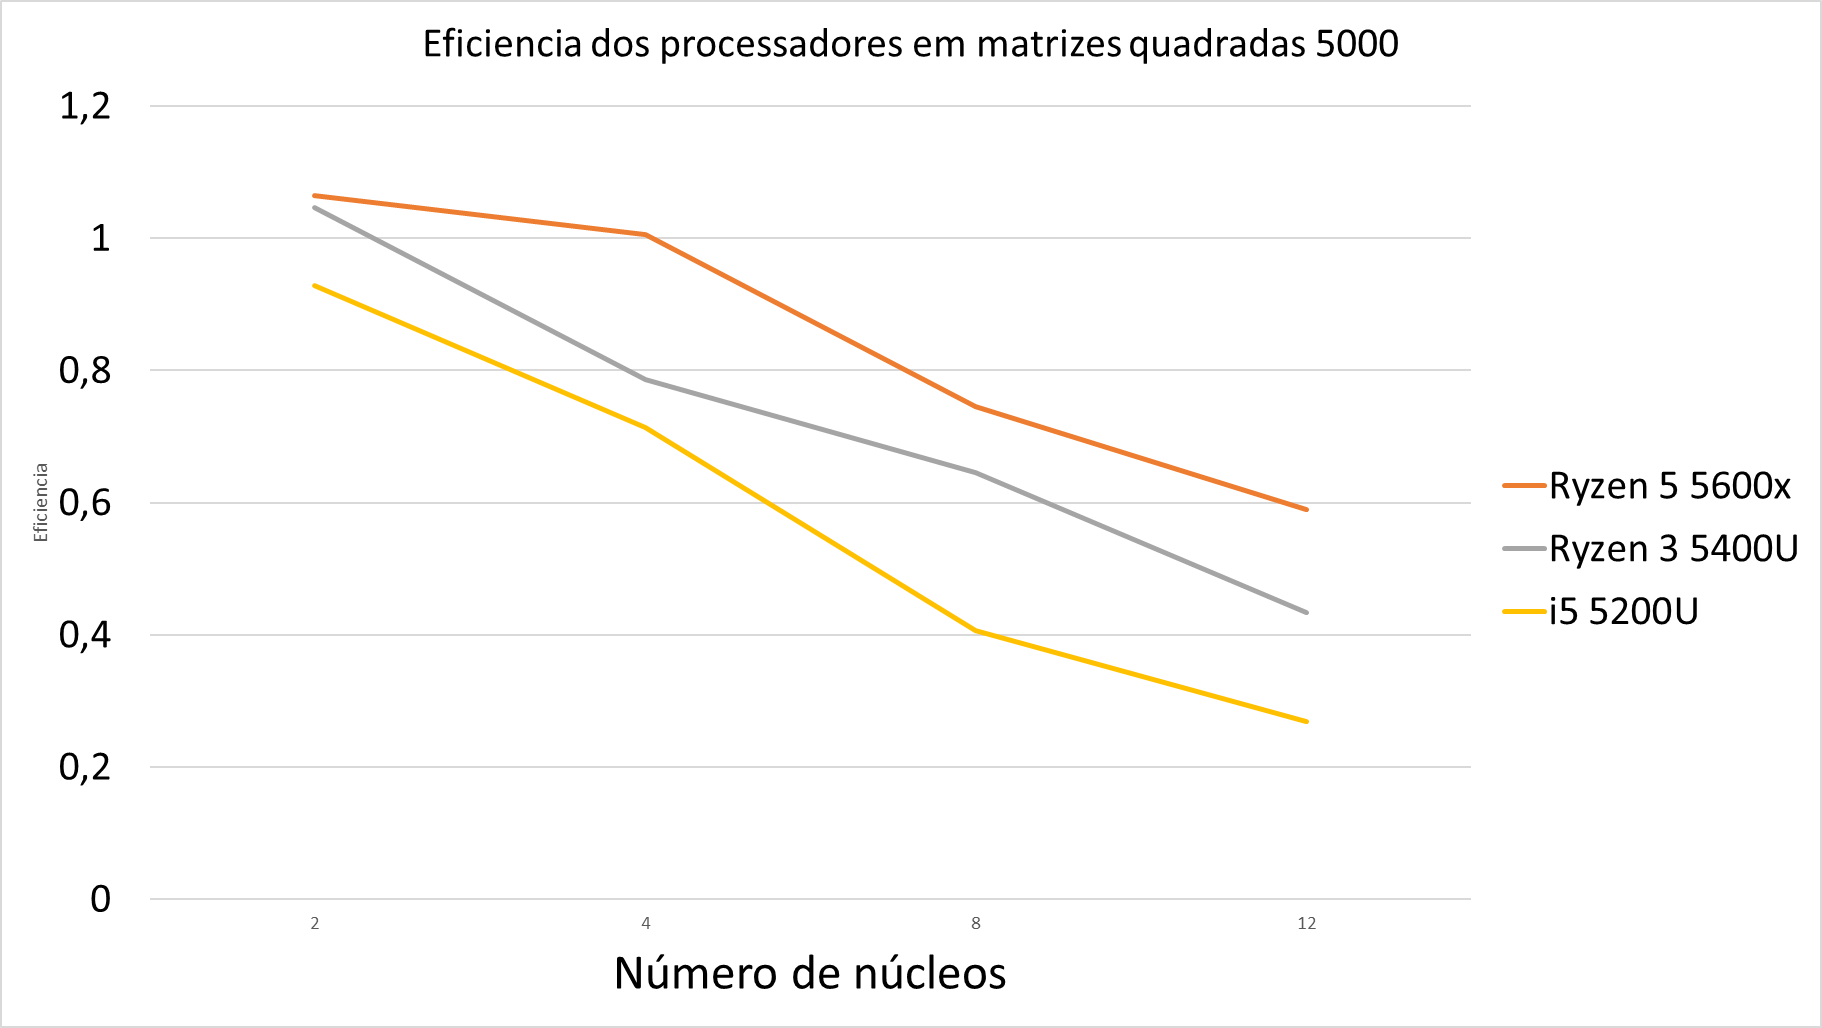
\includegraphics[width=2.5in]{eficiencia-5000.png}}%
\newline Figura 5. Gráfico de eficiência de cada processador para matriz de tamanho 5000
\label{fig:diagrama}

\label{fig:est}
\hfil
\label{fig:est}

\end{figure}
\section{Conclusão}
Com os resultados obtidos, foi possível alcançar um nível relativamente satisfatório em relação ao speedup devido a sua proximidade a linha ideal em estágios iniciais. No entanto, após todos os testes realizados, também é possível concluir que um maior número de threads não necessariamente implica em um maior desempenho. \par \quad Em todos os gráficos de speedup, foi possível notar que, após atingir um número máximo de threads de determinado processador, o ganho de desempenho praticamente não existe mais e, às vezes até diminui. Isso ocorre porque, a partir do momento em que o processador atinge o máximo de threadsdisponíveis, ele começa a intercalar os threads e, a paralelização não faz mais tanto sentido.
\par \quad Nota-se também que, independentemente do tamanho da matriz, a eficiência diminui à medida que mais processadores são usados. Isso pode ser devido ao fato de que, quanto mais processadores são utilizados, a complexidade da divisão de trabalho entre eles se torna muito alta, reduzindo então seu tempo dedicado a resolver o problema.



% if have a single appendix:
%\appendix[Proof of the Zonklar Equations]
% or
%\appendix  % for no appendix heading
% do not use \section anymore after \appendix, only \section*
% is possibly needed

% use appendices with more than one appendix
% then use \section to start each appendix
% you must declare a \section before using any
% \subsection or using \label (\appendices by itself
% starts a section numbered zero.)
%

% use section* for acknowledgment




\bibliographystyle{ieeetr}  %%%% https://www.overleaf.com/learn/latex/bibtex_bibliography_styles

\bibliography{Referências}
Pacheco, P. (2011). An Introduction to Parallel Programming. Morgan Kaufmann Publishers.

SS Wiki. (n.d.).Parallel efficiency - simple approach. Universidade de Magdeburg. Acesso em 15/07/2023, https://wikis.ovgu.de/lss/doku.php?id=guide:parallel_efficiency.

% Can use something like this to put references on a page
% by themselves when using endfloat and the captionsoff option.
\ifCLASSOPTIONcaptionsoff
  \newpage
\fi


%\begin{thebibliography}{1}

%\bibitem{IEEEhowto:kopka}
%H.~Kopka and P.~W. Daly, \emph{A Guide to \LaTeX}, 3rd~ed.\hskip 1em plus
%  0.5em minus 0.4em\relax Harlow, England: Addison-Wesley, 1999.
%
%\end{thebibliography}


\end{document}


